\documentclass{article}
\usepackage[utf8]{inputenc}
\usepackage[portuges]{babel}
\usepackage{csquotes}
\usepackage{geometry}
\usepackage{indentfirst}
\usepackage{graphicx}
\usepackage{float}
\usepackage[pdftex]{hyperref}
\usepackage[backend = biber]{biblatex}
\addbibresource{referencias.bib}
\geometry{top = 3cm, bottom = 2cm, left = 3cm, right = 2cm}

\title{Banco de Dados}
\author{Anne Beatriz Cardoso \\ Igor Cortes Junqueira \\ Igor Patrício Michels \\ João Vinícius Primaki Prado}
\date{2020.2}

\begin{document}
	
	\maketitle
	
	\section{Introdução}
	
	O presente documento tem por objetivo relatar o desenvolvimento da elaboração de um banco de dados para a primeira avaliação da disciplina de Banco de Dados da FGV-EMAp, ministrada pelo professor Renato Rocha Souza. O objetivo inicial era a criação de um banco de dados sobre o tema comida, entretanto, após algumas conversas entre o grupo e autorização do professor, trocou-se para a elaboração de um banco de dados com informações sobre os voos domésticos dos EUA entre janeiro de 2019 e maio de 2020. A escolha por tal período foi feita para possibilitar comparações do pré e pós pandemia nos EUA. Os arquivos utilizados, bem como os script's elaborados podem ser encontrados em \cite{github}.
	
	\section{Elaboração}
	
	\subsection{Fontes}
	
	Os dados dos voos utilizados foram obtidos por meio dos registros oficiais da BTS - Bureau of Transportation Statistics \cite{BTS}, já os dados das aeronaves foram obtidos pelos registros da FAA - Federal Aviation Administration \cite{FAA}.
	
	\subsection{Modelagem Inicial}
	
	Após decidir o tema com o qual iríamos trabalhar, partimos para a elaboração dos modelos conceitual e lógico. A ideia dessa etapa é a de ver como as tabelas de nosso banco irão se relacionar, bem como quais dados podem ser trabalhados de forma a compactar o banco e, ao mesmo tempo, deixar o banco seguindo a forma normal.
	
	\subsubsection{Modelo Conceitual}
	
	Na primeira parte dessa etapa criamos o modelo conceitual, ou seja, vimos como nossas tabelas irão se relacionar. Esse modelo pode ser encontrado na figura \ref{conceitual}.
	\begin{figure}
		\centering
		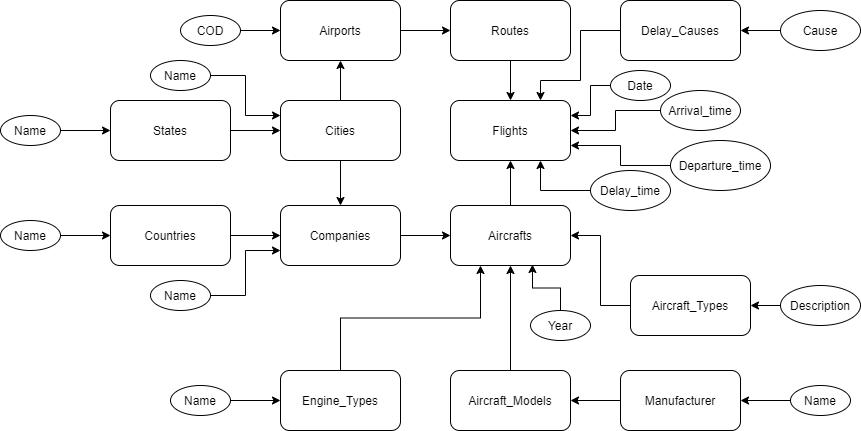
\includegraphics[scale = 0.5]{Imagens/modelo conceitual anterior.png}
		\caption{Modelo Conceitual inicial}
		\label{conceitual}
	\end{figure}
	
	\subsubsection{Modelo Lógico}
	
	Após termos elaborado o modelo conceitual fomos a segunda parte dessa etapa, ou seja, partimos para a elaboração do modelo lógico, conforme podemos ver na figura \ref{lógico}.
	\begin{figure}
		\centering
		\includegraphics[scale = 0.7]{Imagens/modelo lógico anterior.png}
		\caption{Modelo Lógico inicial}
		\label{lógico}
	\end{figure}
	
	\subsection{Extração dos dados}
	
	Para a extração dos dados da BTS simplesmente acessamos o site e baixamos os dados completos, mês a mês, de janeiro 2019 a maio de 2020\footnote{O site não possuía registros mais recentes.}, feito isso, obtivemos um total de 3,26 GB de registros, tudo em 17 arquivos csv, conforme podemos ver na figura \ref{print}.
	\begin{figure}[H]
		\centering
		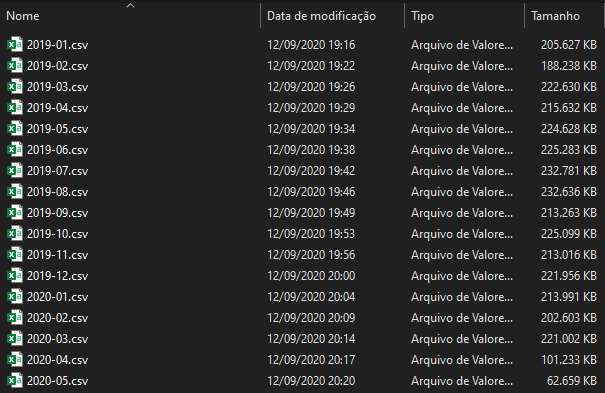
\includegraphics[scale = 0.5]{Imagens/Arquivos.png}
		\caption{Print dos arquivos}
		\label{print}
	\end{figure}
	
	Após isso, precisamos buscar os dados das aeronaves. Assim, pelos registros dos voos pegamos os registros de cada aeronave utilizada e buscamos os respectivos registros no site da FAA.
	
	Como a FAA não libera um arquivo com os dados das aeronaves, mas sim uma página com os dados das aeronaves, elaboramos um script para fazer a busca e coleta dos dados das aeronaves utilizadas. Para utilizar tal script também foi elaborado um arquivo .txt com todos os registros de aeronaves encontrados nos registros da BTS. Durante a execução desse script ocorreram alguns erros de leitura, pois nem todas as aeronaves possuíam registro ativo na FAA.
	
	Para contornar esse problema, criamos uma lista de ``falhas''. Houveram, de um total de 5998 aeronaves, 70 com falha na coleta\footnote{Aeronaves sem registro ou sem registro ativo.}. Dessas falhas, reformulamos o script e o executamos novamente para realizar a coleta dos dados, dessa forma conseguimos coletar os dados de 40 aeronaves com registro vencido, as outras 30 não possuíam registro na FAA, então ficaram sem dados de fabricante, companhia, etc.
	
	A saída desse script foi dada pela geração de 6 arquivos csv, cada um correspondendo a uma tabela do banco (``aircraft\_model'', ``aircraft\_types'', ``aircrafts'', ``companies'', ``engine\_types'' e ``manufacturers''), o que já adiantou parte da manipulação necessária para a criação do banco de dados.
	
	\subsection{Manipulação}
	
	Tendo todos os registros extraídos, precisamos manipular os dados para inseri-los no banco. Conforme comentado anteriormente, os dados obtidos pela FAA já estavam praticamente prontos, entretanto os dados obtidos pela BTS ainda estavam em csv's com diversos dados, muitos que acabavam sendo irrelevantes para a modelagem, então criamos um script para gerar novos csv's, mas apenas com os dados que iríamos utilizar.
	
	Após isso, precisamos manipular esses csv's de forma a separar os dados em arquivos menores, equivalentes as tabelas do banco de dados a ser implementado. Para isso, primeiramente separamos os dados que continham alguma informação acerca dos aeroportos, dessa forma seria mais simples montar as tabelas ``routes'', ``airports'' e ``cities''\footnote{Essa última de forma parcial.}.
	
	Com a modelagem descrita acima, percebemos que havia apenas um registro de aeroporto/companhia fora dos EUA, dessa forma optamos por ignorar tal registro, mantendo apenas os voos domésticos, conforme planejado inicialmente. Com essa decisão, a tabela ``country'' foi excluída, uma vez que todos são referentes aos EUA. Além dessa exclusão, fizemos algumas outras alterações no banco como, por exemplo, a retirada do nome dos aeroportos. Feito isso, obtivemos os modelos que podem ser encontrados nas figuras \ref{new_conceitual} e \ref{new_lógico}.
	\begin{figure}
		\centering
		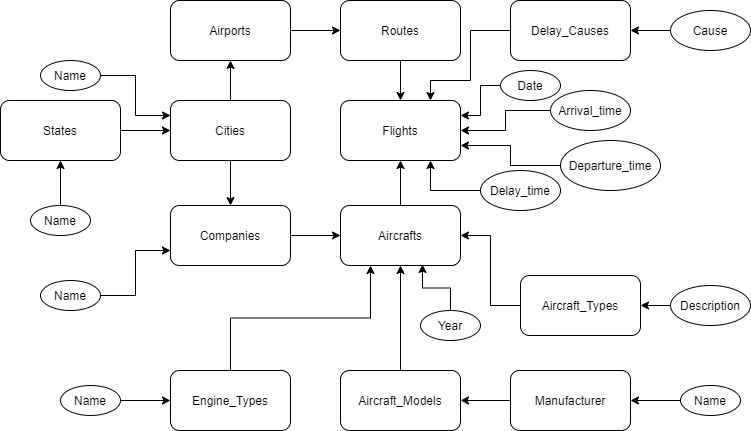
\includegraphics[scale = 0.5]{Imagens/modelo conceitual.png}
		\caption{Novo Modelo Conceitual}
		\label{new_conceitual}
	\end{figure}
	
	\begin{figure}
		\centering
		\includegraphics[scale = 0.7]{Imagens/modelo lógico.png}
		\caption{Novo Modelo Lógico}
		\label{new_lógico}
	\end{figure}
	
	Para finalizar a modelagem dessas tabelas mais simples foi utilizada uma solução manual, fazendo todas as referências entre as tabelas através do Excel com o PROCV. A ideia de fazer manualmente se deu em virtude de haver muitos dados de cidades e companhias sem um padrão: a cidade de Atlanta tinha, além desse registro, os registros de Allanta e Altanta, por exemplo. Já a tabela ``Delay\_Causes'' a solução manual se deu por serem apenas quatro registros, os quais eram labels de colunas dos nossos dados. Nas demais tabelas foi, basicamente, colocado a ID, quando necessária, e referenciado os dados com outras tabelas, com exceção da ``states'', a qual considera todos os estados dos EUA, os quais podem ser encontrados em uma lista online como, por exemplo, na Wikipédia.
	
	Com o procedimento anterior já havíamos finalizado quase todas as tabelas, com exceção a tabela ``flights'', a qual requer um cuidado maior com o preenchimento do campo ``Delay\_Causes\_id''. Para contornar esse problema criamos um código para ver qual das causas de delay gerou o maior atraso no voo, dessa forma, conseguimos encontrar a ``causa do delay''. Após isso, faltou apenas referenciar o voo com a rota, o que também foi feito no Excel.
	
	Após realizar todo processo descrito acima, criamos o banco e, em seguida, elaboramos um script para fazer a inclusão dos dados que se encontravam nos csv's para o banco de dados.
	
	\section{Resultados}
	
	Um primeiro resultado interessante já pôde ser observado na figura \ref{print}. Lá pudemos ver, na última coluna, que o tamanho dos arquivos diminuiu muito nos meses de abril e maio de 2020 quando comparado aos demais meses, em especial no mesmo período de 2019, ou seja, os estadunidenses passaram a viajar menos e, com isso, o arquivo passou a ter menos dados. Isso já se mostrou ser um dos reflexos do coronavírus, uma vez que a população passou a ficar mais isolada.
	
	Já o resultado final, isto é, o banco de dados, pode ser encontrado \href{https://gvmail-my.sharepoint.com/:f:/g/personal/b39254_fgv_edu_br/Ev8i0xwOqnFFh_q3gTqvNAkBhzL_dpV6_ljzh82vJsTnNg?e=7ubrsl}{\textbf{nesse link}}.
	
	\printbibliography
	
\end{document}
